% !TEX TS-program = pdflatex
% Beamer slide deck for the ConcatCIFAR10 modular-FC experiments.
% Figures are produced by the scripts in this folder; run ./build_figures.sh
% first, then compile with:  pdflatex slides.tex
\documentclass[aspectratio=169]{beamer}

\usepackage{graphicx}
\usepackage{amsmath, amssymb}
\usepackage{booktabs}
\usepackage{xcolor}

\graphicspath{{figs/}}

\usetheme{default}
\usecolortheme{seagull}
\setbeamertemplate{navigation symbols}{}
\setbeamertemplate{footline}[frame number]
\setbeamerfont{frametitle}{size=\large,series=\bfseries}

\newcommand{\code}[1]{\texttt{\small #1}}

\title{Driving modular FC connectivity via\\ a weighted-activity regularizer}
\subtitle{ConcatCIFAR10 with a ResNet-18 trunk\\
  \small (batch size 128, reg\_weight 1.0, 100 epochs)}
\author{}
\date{\today}

\begin{document}

% --- 1. Title -----------------------------------------------------------
\begin{frame}
  \titlepage
\end{frame}

% --- 2. Motivation ------------------------------------------------------
\begin{frame}{Motivation: split one network into N independent sub-networks}
  \begin{columns}[T]
    \column{0.55\textwidth}
    \textbf{Task.} Concatenate $N$ CIFAR-10 frames horizontally; ask one
    network to classify all $N$ simultaneously.
    \medskip

    \textbf{Goal.} Train the FC head so that it factorises into $N$
    independent sub-networks --- one per frame --- without hardcoding the
    split.
    \medskip

    \textbf{Tool.} A weighted-activity regularizer on the hidden layer that
    penalises every hidden unit by the squared magnitudes of its
    outgoing \code{fc2} connections.

    \column{0.45\textwidth}
    \textbf{Why this question?}
    \begin{itemize}\setlength\itemsep{3pt}
      \item Test whether a simple training-time inductive bias can recover
        the block structure that the task implies.
      \item Quantify how quickly modularity emerges, and how it scales with
        the number of modules $N$.
      \item Read modularity directly off \code{fc2} via the Laplacian
        spectrum --- no clustering required to define the metric.
    \end{itemize}
  \end{columns}
\end{frame}

% --- 3. Task ------------------------------------------------------------
\begin{frame}{The task: \texttt{ConcatCIFAR10}}
  \centering
  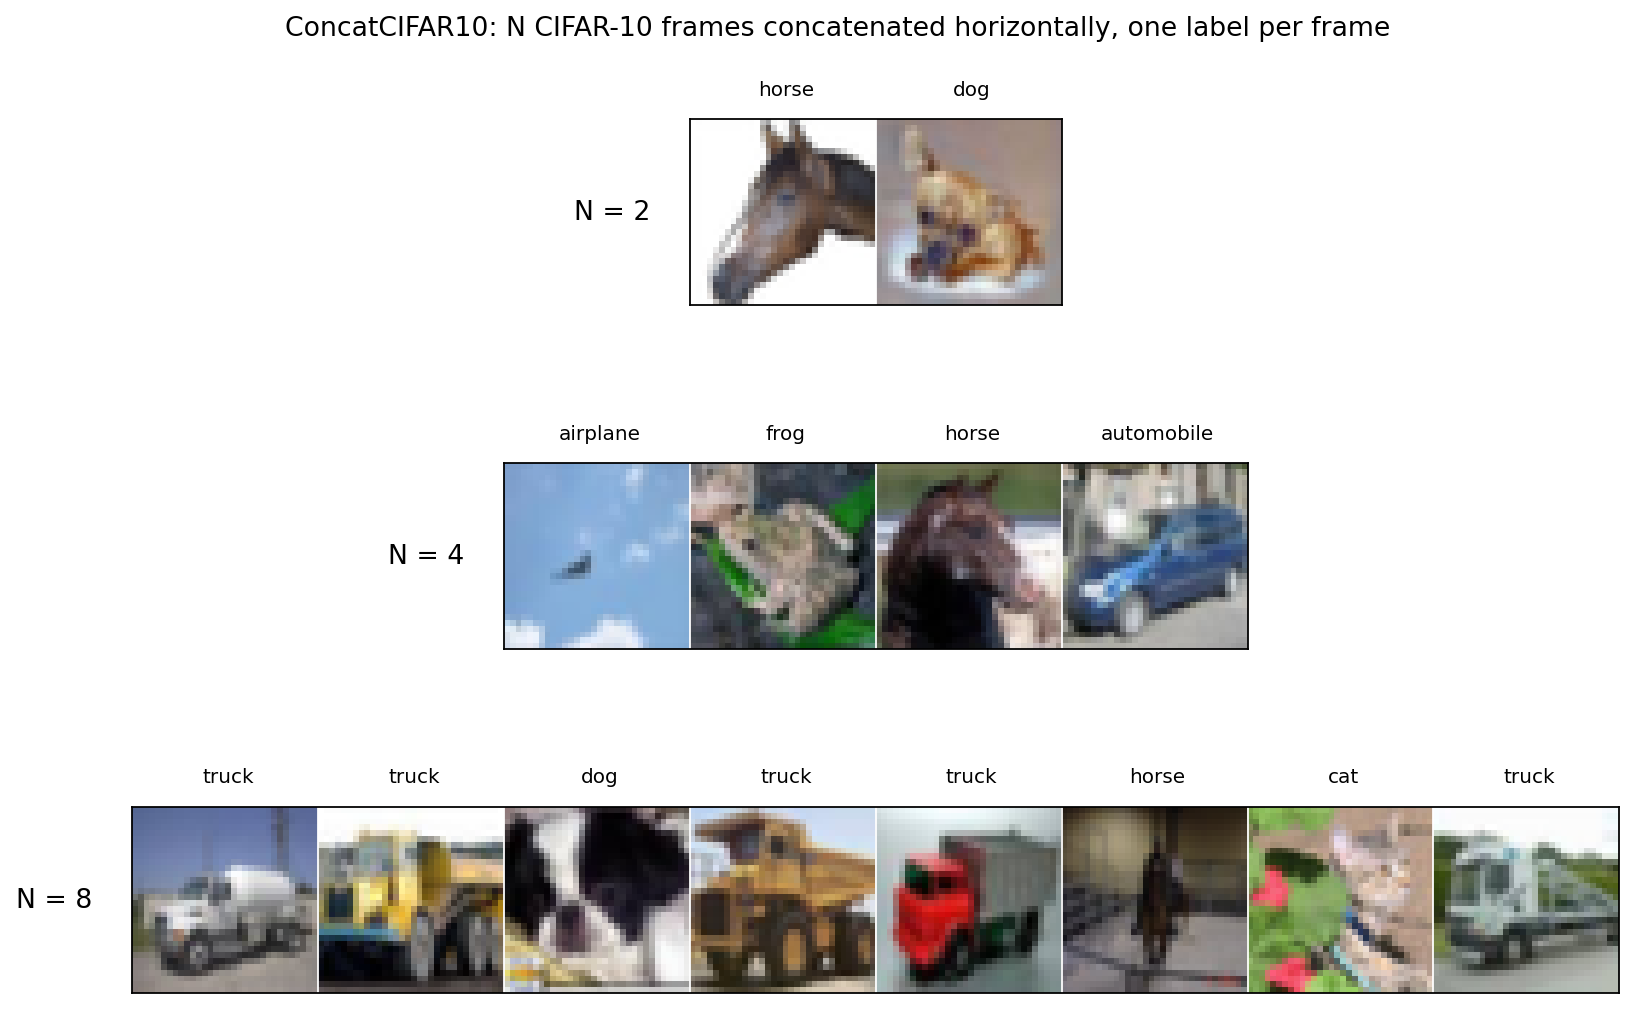
\includegraphics[width=0.92\linewidth]{task_examples}
  \begin{itemize}\small
    \item Input shape $(3, 32, 32N)$; per-sample label is a length-$N$
      vector.
    \item Frames drawn i.i.d.\ inside \code{\_\_getitem\_\_} --- same
      index returns a different concatenation on each access.
    \item Each frame is irrelevant context for the other $N-1$ outputs.
  \end{itemize}
\end{frame}

% --- 4. Architecture ----------------------------------------------------
\begin{frame}{Architecture: ResNet-18 trunk $+$ per-frame MLP head}
  \centering
  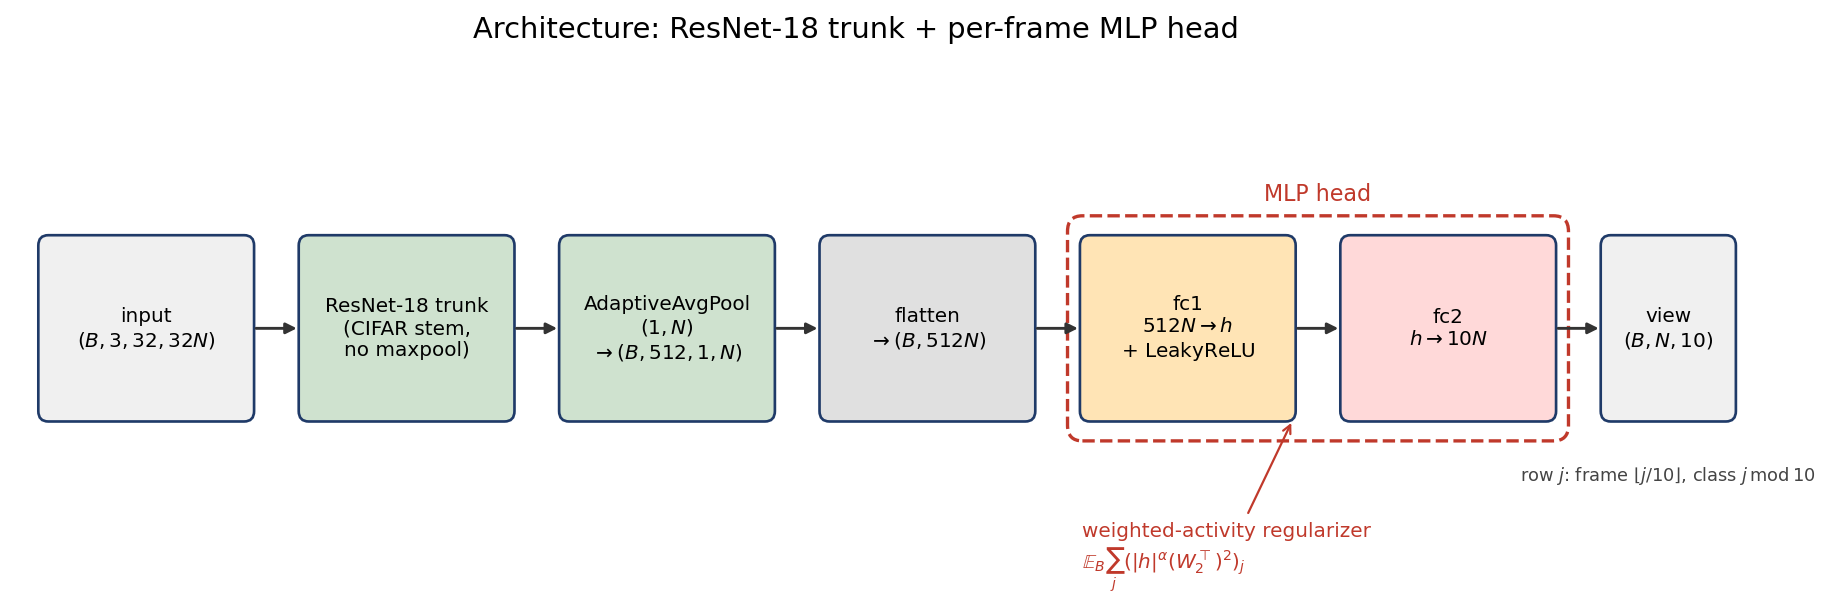
\includegraphics[width=0.98\linewidth]{arch_pipeline}
  \begin{itemize}\small
    \item CIFAR adaptation of ResNet-18 (3$\times$3 stem, no maxpool).
    \item \code{AdaptiveAvgPool((1,N))} keeps one position per frame along
      the width.
    \item MLP head: $512N \to h \to 10N$, default $h{=}512N$, LeakyReLU(0.1).
    \item Regularizer attaches to the \emph{hidden activation}, using
      \code{fc2} weights --- single-layer version is trivial.
  \end{itemize}
\end{frame}

% --- 5. Regularizer + readout pipeline ---------------------------------
\begin{frame}{Modularity readout: Laplacian spectrum of $|W_{fc2}|$}
  \centering
  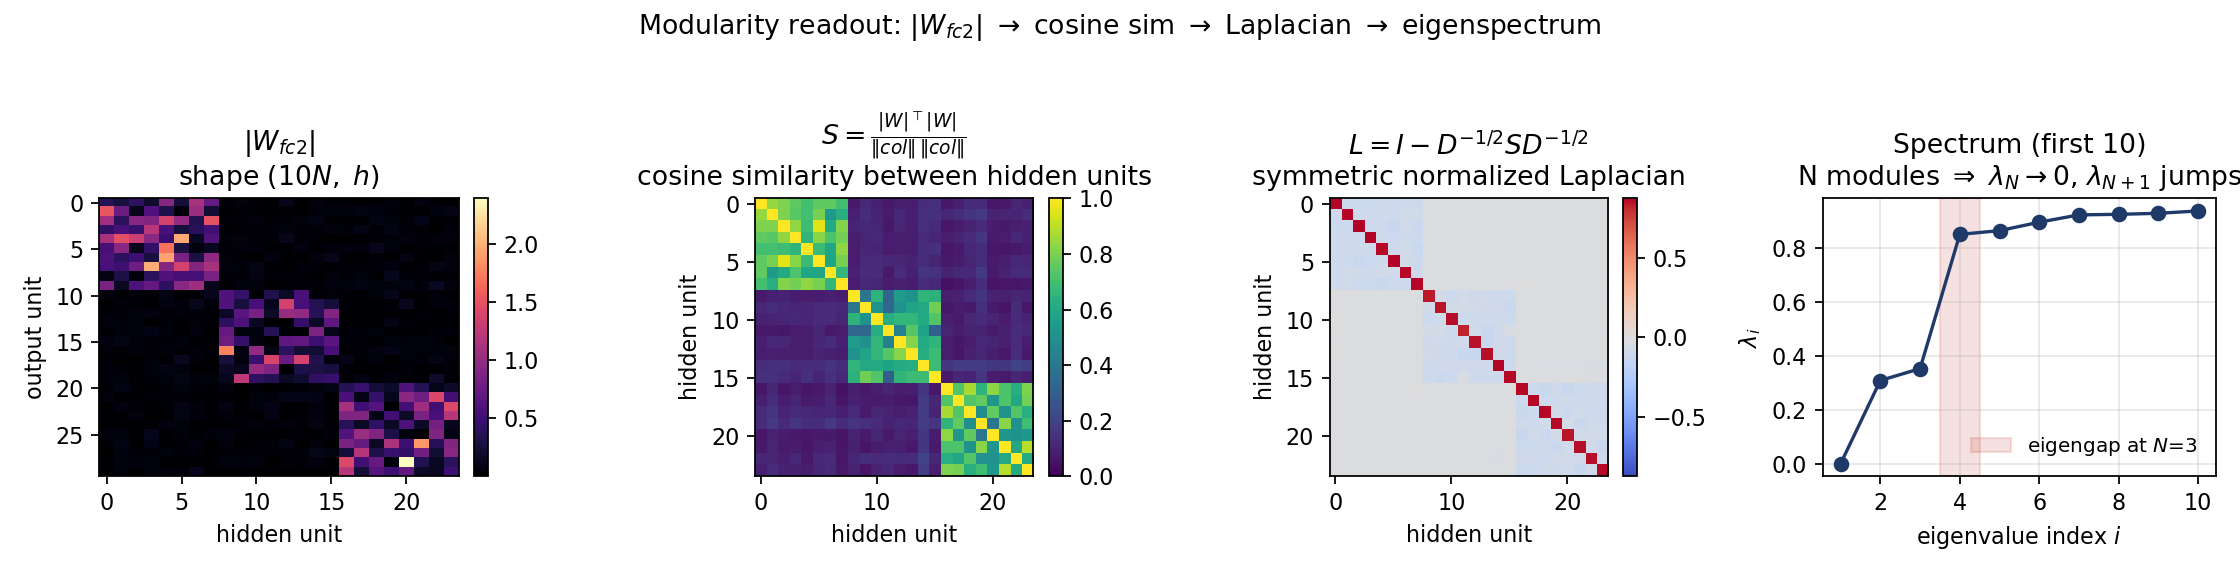
\includegraphics[width=0.98\linewidth]{modularity_pipeline}
  \vspace{-0.5em}
  \begin{itemize}\small
    \item Nodes are hidden units; edge weight $S_{ij}$ is cosine similarity
      of their \emph{outgoing} $|W_{fc2}|$ columns.
    \item Symmetric normalized Laplacian $L = I - D^{-1/2} S D^{-1/2}$ has
      the same spectrum as the random-walk Laplacian used in
      \code{modularisation\_via\_noise/utils/graphs.py}.
    \item $N$ disconnected modules $\Rightarrow$ first $N$ eigenvalues
      $\approx 0$, eigengap at position $N$.
  \end{itemize}
\end{frame}

% --- 6. Training accuracy ----------------------------------------------
\begin{frame}{Sanity check: all $N$ values learn (sort of)}
  \centering
  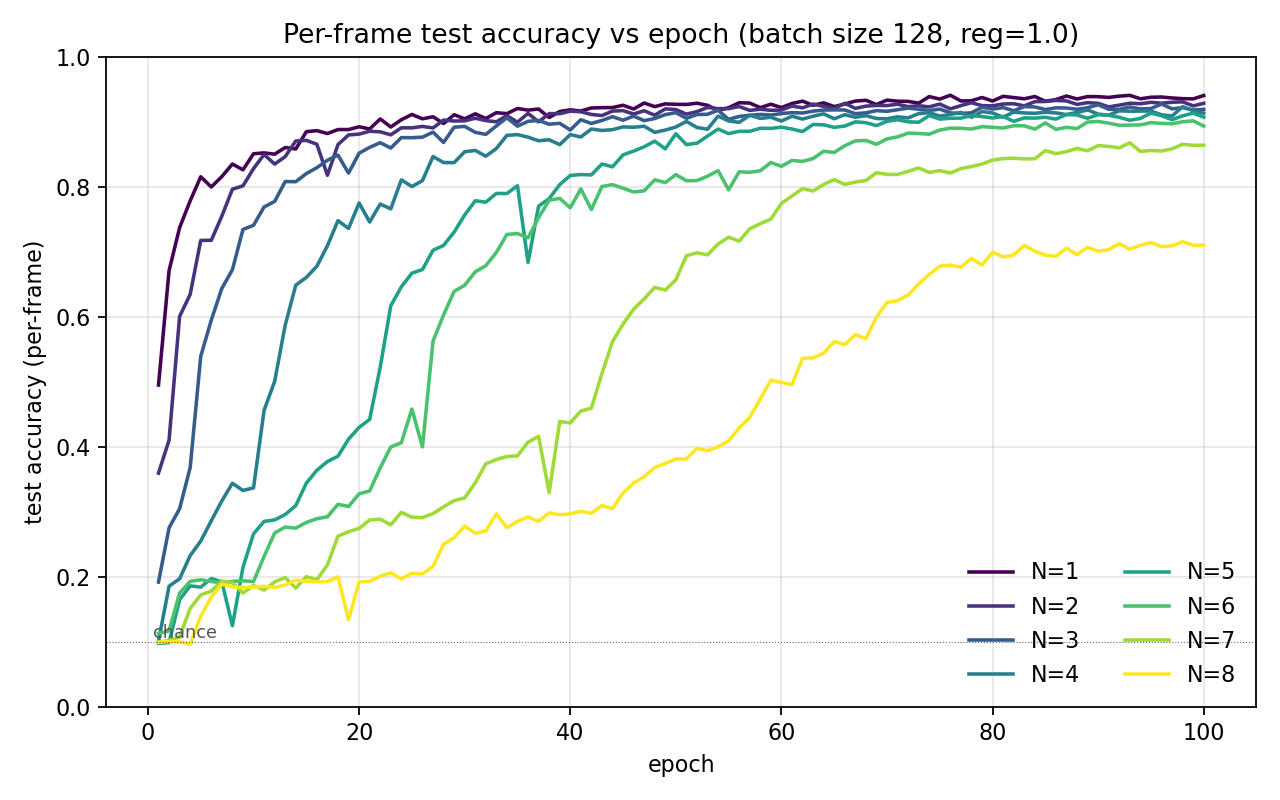
\includegraphics[width=0.72\linewidth]{training_accuracy}
  \begin{itemize}\small
    \item Final per-frame test accuracy: $N{=}1$: 0.94 down to $N{=}8$: 0.71.
    \item $N{\le}6$ converge cleanly; $N{=}7,8$ are still rising at epoch 100.
    \item Difficulty scales with $N$ --- the trunk has to keep $N$ frames
      separable at the hidden layer.
  \end{itemize}
\end{frame}

% --- 7. Representative eigenvalue trajectories --------------------------
\begin{frame}{Eigenvalue trajectories: first 10 of fc2 (N = 4 run)}
  \centering
  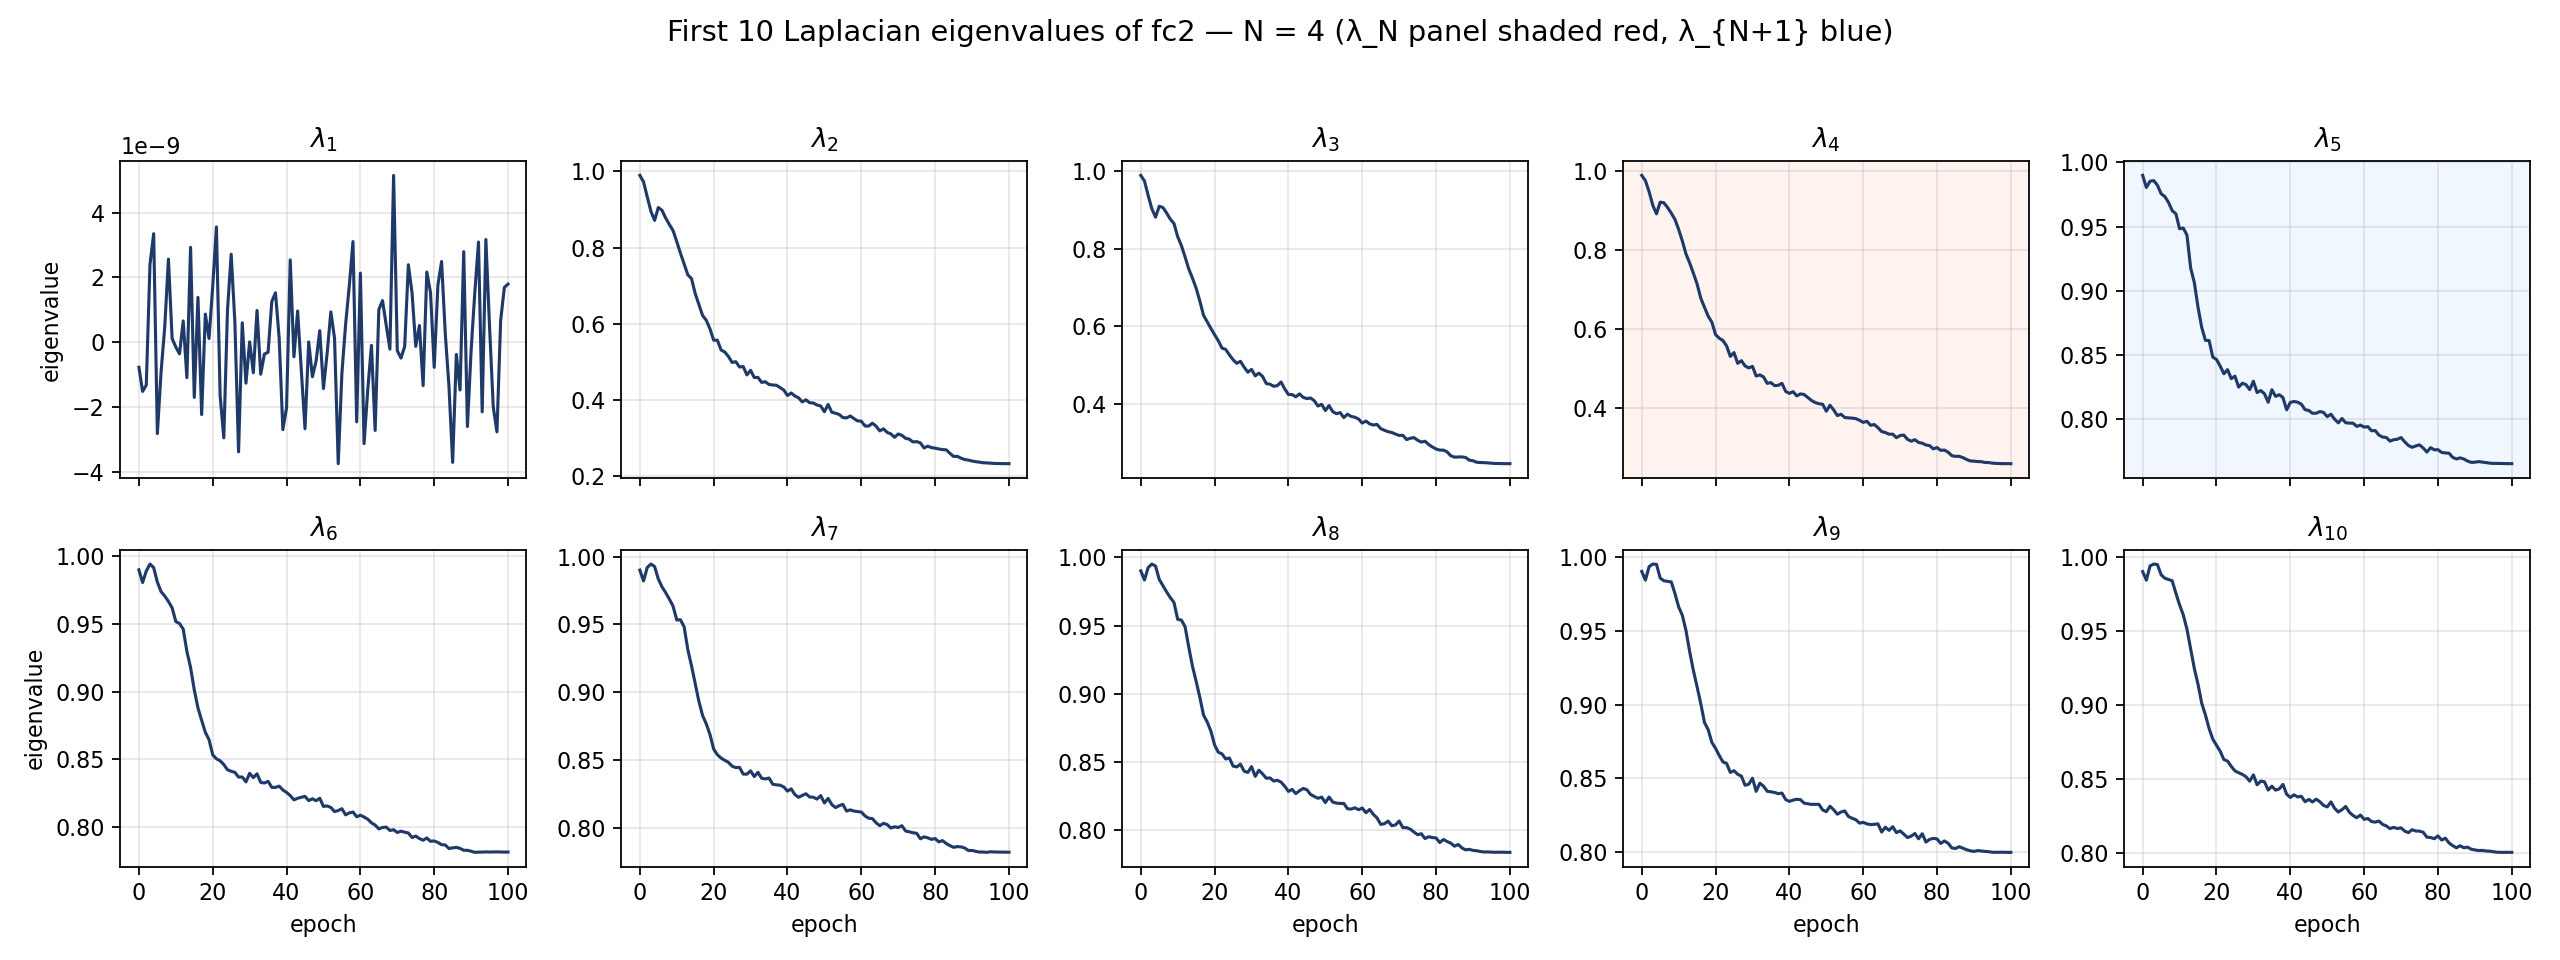
\includegraphics[width=0.96\linewidth]{eigvals_representative}
  \begin{itemize}\small
    \item $\lambda_1 \equiv 0$ (a connected component is always present
      modulo numerical noise).
    \item $\lambda_2 \ldots \lambda_4$ all collapse toward 0 --- emergence
      of $N{=}4$ disconnected components.
    \item $\lambda_5$ stays well above 0: eigengap opens at position $N$.
  \end{itemize}
\end{frame}

% --- 8. lambda_N and lambda_{N+1} overlay ------------------------------
\begin{frame}{$\lambda_N$ and $\lambda_{N+1}$ across $N$}
  \centering
  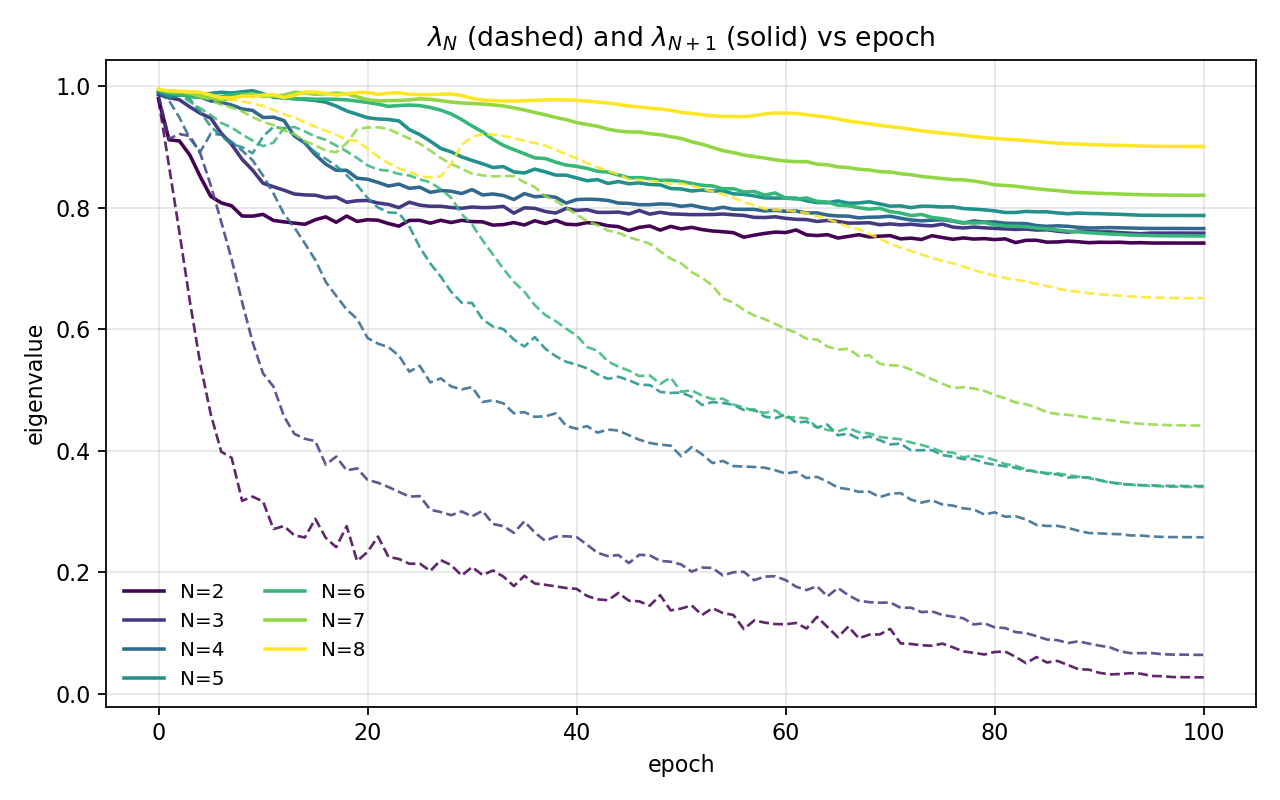
\includegraphics[width=0.78\linewidth]{lamN_pair}
  \begin{itemize}\small
    \item Solid: $\lambda_{N+1}$ (should stay high). Dashed: $\lambda_N$
      (should fall toward 0).
    \item Gap visibly opens for every $N\ge 2$; for $N{=}8$ the gap is much
      narrower at the end of training.
  \end{itemize}
\end{frame}

% --- 9. Cross-N eigengap dynamics --------------------------------------
\begin{frame}{Eigengap dynamics: how does emergence scale with $N$?}
  \centering
  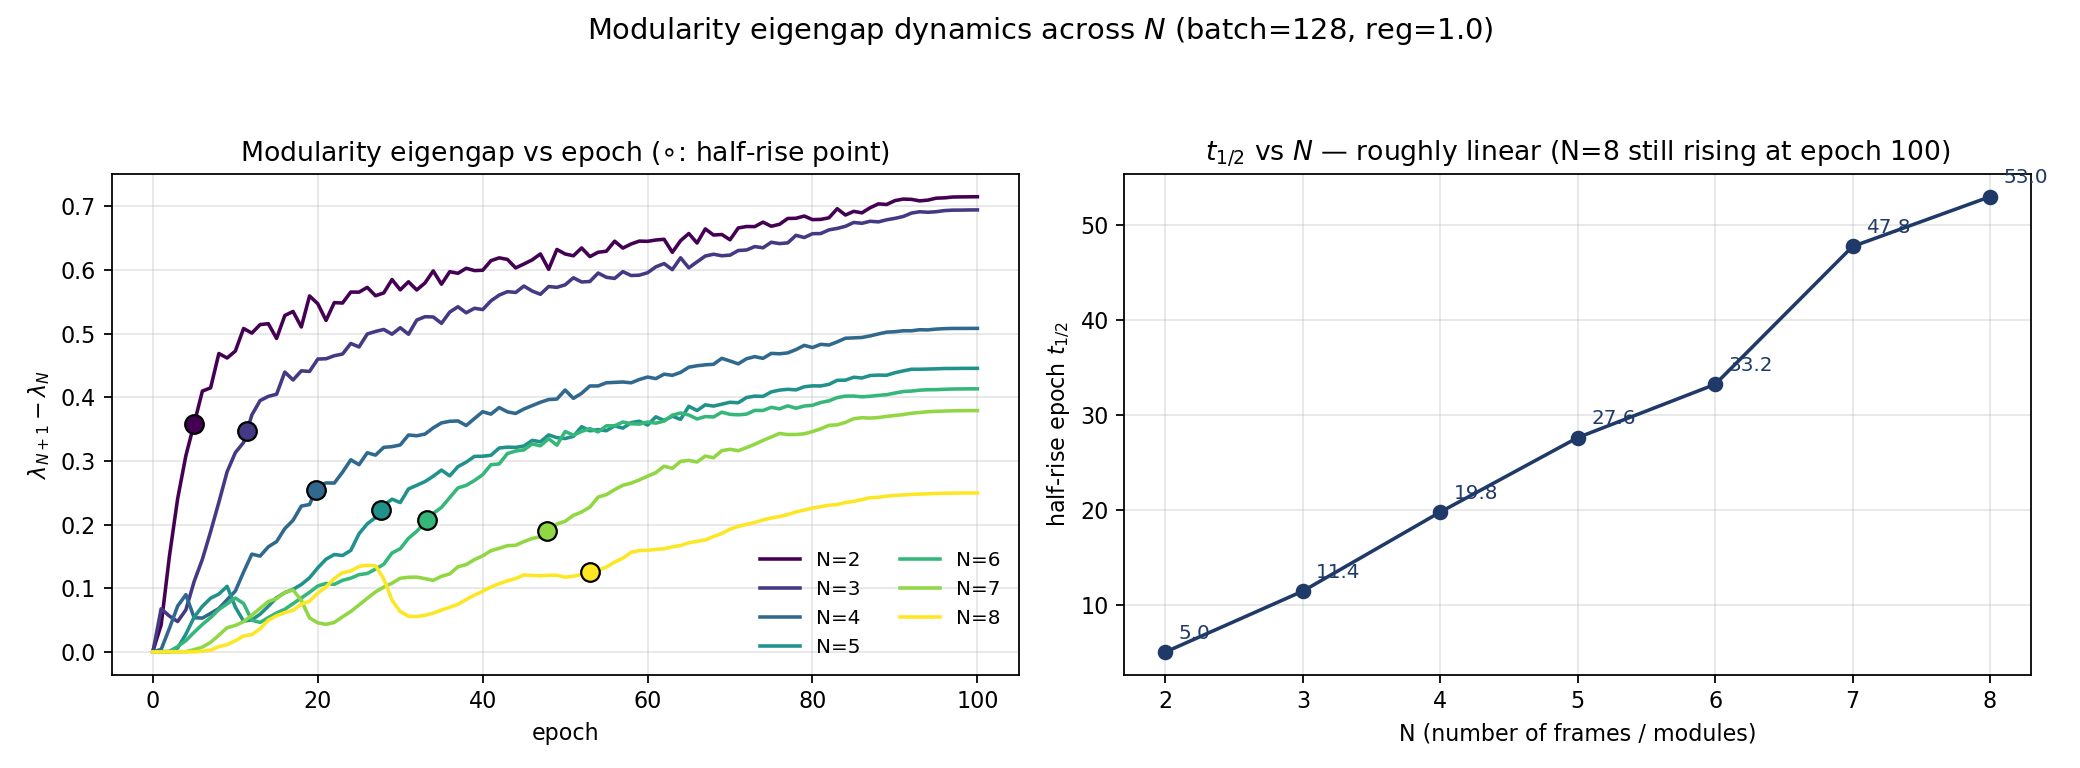
\includegraphics[width=0.96\linewidth]{eigengap_overview}
  \begin{itemize}\small
    \item Left: per-$N$ gap trace with the half-rise point
      $(t_{1/2}, g_{1/2})$ overlaid; $g_{1/2} \equiv (g_{\mathrm{init}} +
      g_{\mathrm{final}})/2$.
    \item Right: $t_{1/2}$ vs $N$ grows roughly linearly --- $\sim$5 epochs
      at $N{=}2$ to $\sim$50 at $N{=}8$.
    \item $N{=}8$ point underestimates --- run hasn't finished rising at
      epoch 100.
  \end{itemize}
\end{frame}

% --- 10. Final-epoch summary -------------------------------------------
\begin{frame}{Final-epoch summary: modularity emerges, but weakens with $N$}
  \centering
  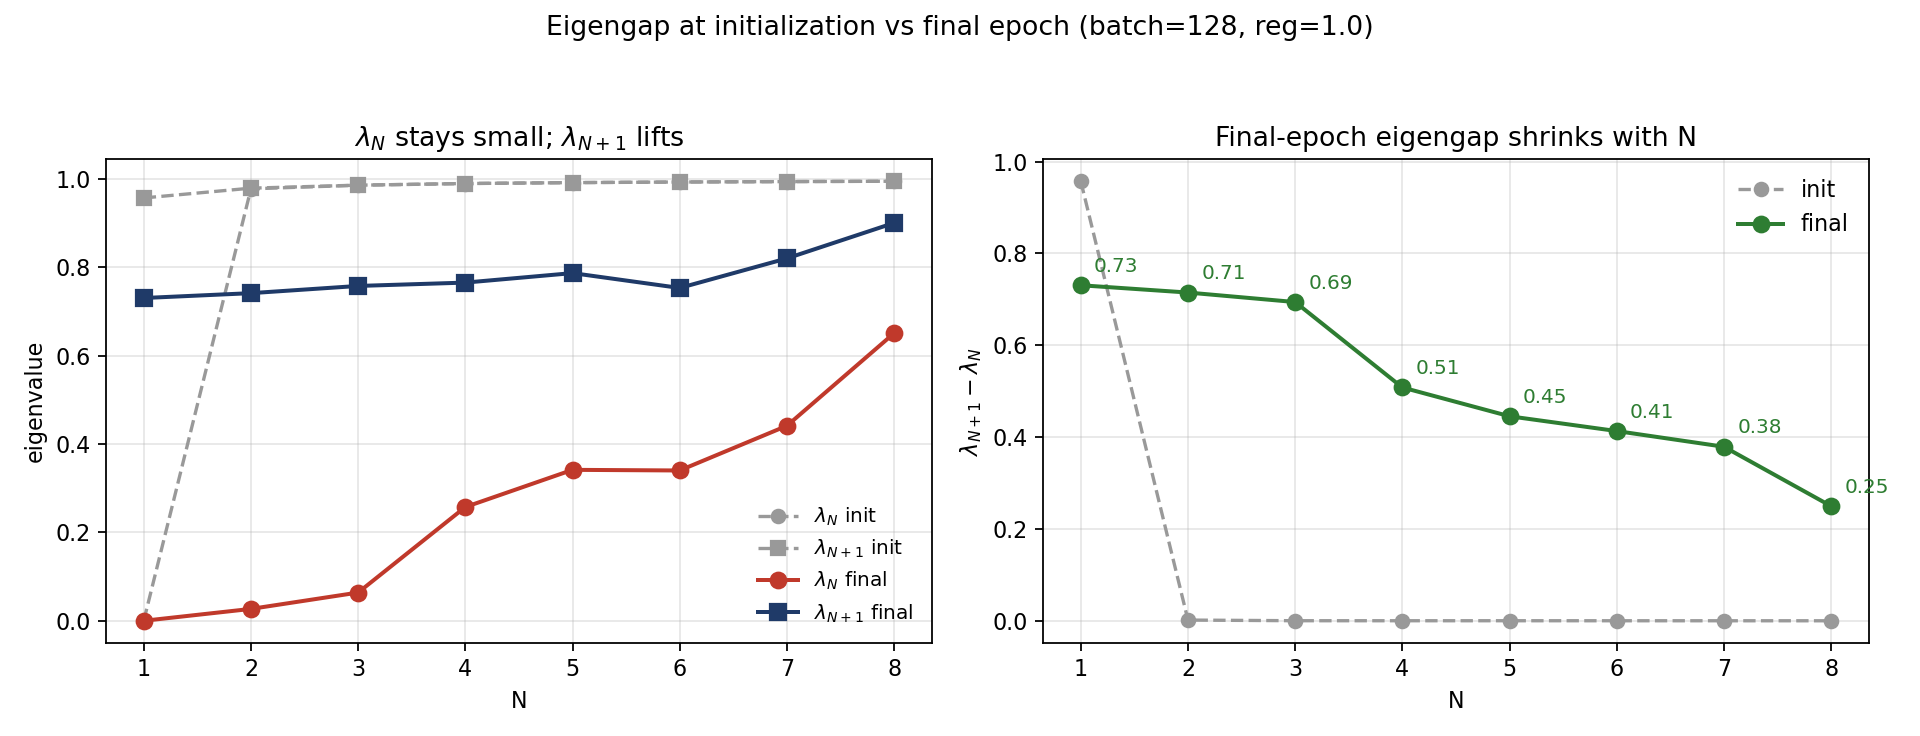
\includegraphics[width=0.92\linewidth]{final_modularity_vs_N}
  \begin{itemize}\small
    \item At init the spectrum is uninformative ($\lambda_N \approx
      \lambda_{N+1}$ for all $N{\ge}2$, gap $\approx 0$).
    \item Training drives $\lambda_N$ small while $\lambda_{N+1}$ stays
      large; final gap shrinks from $\sim$0.71 ($N{=}2$) to $\sim$0.25
      ($N{=}8$).
  \end{itemize}
\end{frame}

% --- 11. Weight visualisation ------------------------------------------
\begin{frame}{Visualising the learned modularity: $|W_{fc2}|$ heatmaps}
  \centering
  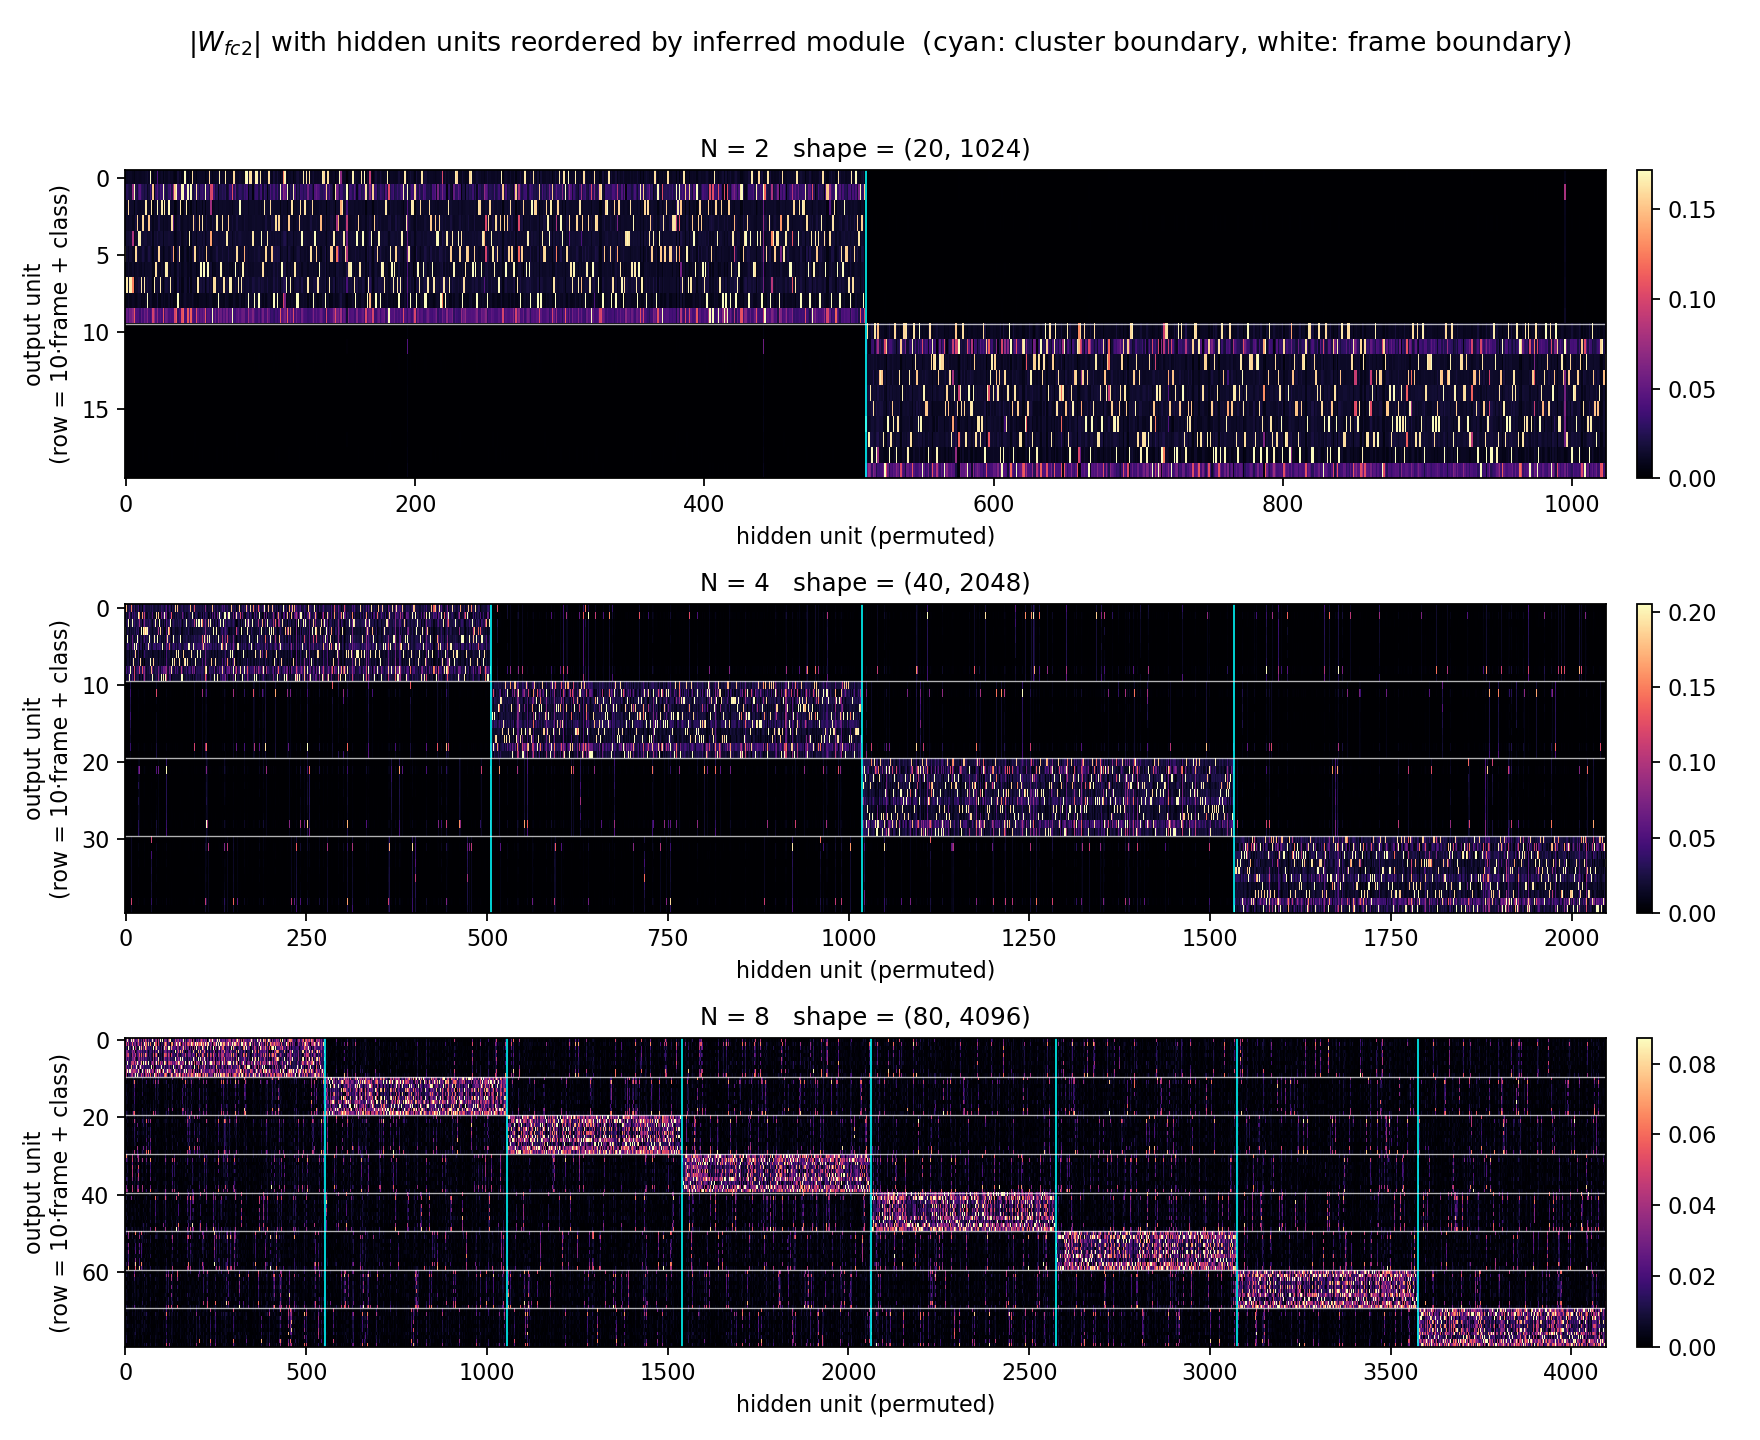
\includegraphics[width=0.78\linewidth]{fc2_heatmaps_grid}
  \begin{itemize}\small
    \item Hidden units (columns) reordered by spectral $k$-means with
      $k{=}N$, then matched to frames by max-affinity assignment.
    \item Cyan: cluster boundary. White: frame boundary ($10$ rows / frame).
    \item Clear block-diagonal structure at $N{=}2, 4$; partial but visible
      at $N{=}8$.
  \end{itemize}
\end{frame}

% --- 12. Summary -------------------------------------------------------
\begin{frame}{Summary and next steps}
  \textbf{What works at batch 128, reg=1.0.}
  \begin{itemize}\setlength\itemsep{2pt}
    \item Weighted-activity regularizer on the hidden layer drives
      \code{fc2} into a block-diagonal structure for $N$ up to $\sim$6
      cleanly, with degraded but still visible modularity at $N{=}7, 8$.
    \item Test accuracy stays close to single-task levels for $N{\le}6$
      (0.89 at $N{=}6$); $N{=}7,8$ haven't fully converged in 100 epochs.
    \item Time to half-modularity grows roughly linearly with $N$; the
      $t/N$ rescaling does not collapse the dynamics.
  \end{itemize}
  \medskip
  \textbf{Open questions / next experiments.}
  \begin{itemize}\setlength\itemsep{2pt}
    \item Batch-size sweep (32, 64): does $t_{1/2}(N)$ slope change?
    \item Reg-weight sweep at fixed $N$: cleanest operating point?
    \item Baseline at reg$=$0 for each $N$ to bound the
      no-regularization modularity.
    \item Alternative regularizers (\code{regularizer\_L12},
      \code{regularizer\_L21} in \code{modularisation\_via\_noise}).
  \end{itemize}
\end{frame}

\end{document}
